                                                                                                                                                                                                                                                                                                                                                                                                                                                                                                                                                                                                                                                                                                                                                                                                                                                                                                                                                                                                                                                                                                                                                                                                                                                                                                                                                                                                      \begin{frame}
\titlepage
\end{frame}
\begin{frame}
\frametitle{Problem Statement-Triangle Exercise}


\begin{enumerate}[label=(\roman*)]
\item ABC and DBC are two triangles on the same
base BC. If AD intersects BC at O, show that\\
$\frac{ar(ABC)}{ar(DBC)}=\frac{AO}{DO}$\\
\end{enumerate}
\textbf{Soln:}\\

\url{https://github.com/Rajolep/_Geometry/blob/master/figs/construc.tex}
\begin{figure}
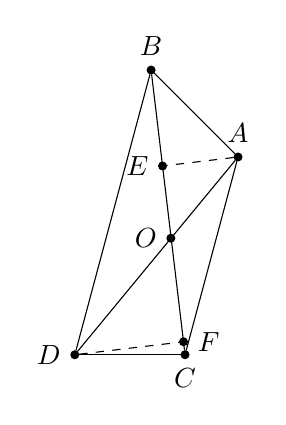
\begin{tikzpicture}
[scale = 0.4,>=stealth,point/.style = {draw, circle, fill = black, inner sep = 1pt},]
\node (A) at (5.1823,6.27851)[point,label=above :$A$] {};
\node (D) at (0,0)[point,label=left :$D$] {};
\node (C) at (3.5,0)[point,label=below :$C$] {};
\node (B) at (2.42196082,9.0388)[point,label=above :$B$] {};
\node (E) at (2.78527772,5.99262965)[point,label=left :$E$] {};
\node (F) at (3.45091219,0.41157955)[point,label=right :$F$] {};
\node (O) at (3.05,3.7)[point,label=left :$O$] {};
\draw (D)--(A);
\draw (A)--(B);
\draw (B)--(C);
\draw (A)--(C);
\draw (B)--(D);
\draw (C)--(D);
\draw [dashed] (A) -- (E);
\draw [dashed] (D) -- (F);
\tkzMarkRightAngle[draw=red,size=.4](A,E,C)
\tkzMarkRightAngle[draw=red,size=.4](D,F,E)
\end{tikzpicture}
\end{figure}
\end{frame}
\begin{frame}
D(0,0)\\
B(2.4219,9.0388)\\
A(5.1823,6.27881)\\
\begin{figure}
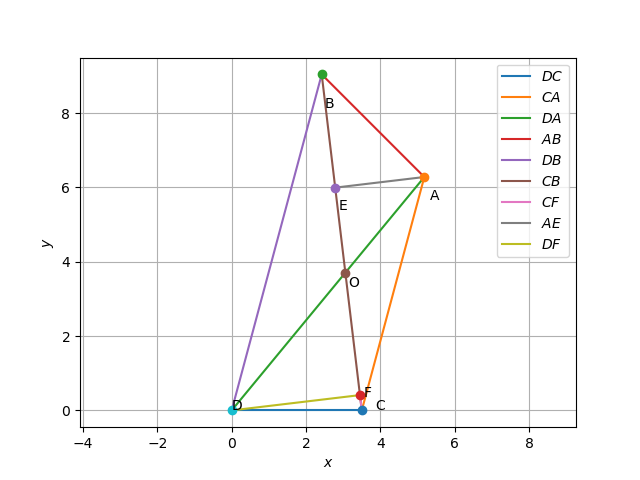
\includegraphics[scale=0.3]{./figs/triexe.png}
\end{figure}
\url{https://github.com/Rajolep/_Geometry/blob/master/codes/triangle/draw_triangle.py}
\end{frame}
\begin{frame}
\begin{align*}
AE\perp BC , DF\perp BC\\
Area of \triangle{ABC} = \frac{1}{2}(BC)(AE)\\
Area of \triangle{DBC} = \frac{1}{2}(BC)(DF)\\
\frac{ar\triangle{ABC}}{ar\triangle{DBC}}=\frac{\frac{1}{2}(BC)(AE)}{\frac{1}{2}(BC)(DF)}\\  
\frac{ar\triangle{ABC}}{ar\triangle{DBC}}=\frac{AE}{DF}\\
\frac{AE}{DF}=\frac{AO}{DO}\\
\angle{AEO}=\angle{DFO}..... RA\\
\angle{AEO}=\angle{DOF}..... VOA\\
\triangle{AOE} \sim \triangle{DOF}\\
\frac{AE}{DF}=\frac{AO}{DO}\\
\end{align*}
\end{frame}
\begin{frame}
\begin{align*}
AE=2.407\\
BC=e=9.10294\\
DF=3.4756\\
AO=AE...(1)\\
DO=DF...(2)\\
\end{align*}
From  (1) and  (2)\\
Area of $\triangle{ABC} = \frac{1}{2}(BC)(AE)  = 38.0739$\\
Area of$ \triangle{DBC} = \frac{1}{2}(BC)(DF)  = 38.0739$\\
\end{frame}